\chapter{Task2}
\section{a)}
If we chose the machine $M$ as follows: $$M = (q_0, \emptyset, \delta, q_0, {q_0})$$
Then it can be proved that the only language accepted by a machine which has only the start state is the empty string $\epsilon$. 
So the second machine would have as complement language $$\Sigma^* \backslash \epsilon \rightarrow \epsilon \backslash \epsilon = \emptyset$$ remembering that $\emptyset^* = \epsilon$.\\
 So this would mean that the machine $M'$ would be something similar to this. 
\begin{center}
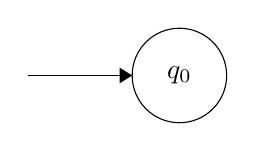
\begin{tikzpicture}[scale=0.2]
\tikzstyle{every node}+=[inner sep=0pt]
\draw [black] (25.5,-26.5) circle (3);
\draw (25.5,-26.5) node {$q_0$};
\draw [black] (15.9,-26.5) -- (22.5,-26.5);
\fill [black] (22.5,-26.5) -- (21.7,-26) -- (21.7,-27);
\end{tikzpicture}
\end{center}
Thus meaning that no language could be accepted by this machine. Since also $M'$ has like acceptance state $Q \backslash F \rightarrow q_0 \backslash q_0 \rightarrow \emptyset$. 
\section{b)}
To disprove the statement, it is enough to show a counterexample. Suppose L contains at least two distinct words $w_1$ and $w_2$, where $w_1$ is not equal to $w_2$. Since $M$ accepts language $L$, there are paths in $M$ that accept $w_1$ and $w_2$. Since $M$ is a NFA, there can be different paths that lead to the same accepting states. Now suppose that $M'$ is an NEA that has exactly one accepting state and $L(M') = L$. Since $L$ contains at least $w_1$ and $w_2$, $M'$ must have paths that accept $w_1$ and $w_2$. Since $M'$ has only one accepting state, these paths must lead to that state. Since $w_1$ and $w_2$ are different words, there is a difference in the paths that accept them. This means that $M'$ is not able to distinguish $w_1$ and $w_2$ and thus is not able to accept L correctly. Therefore, there cannot be an NEA $M'$ with exactly one accepting state such that $L(M') = L$.
An example for this is a machine that accepts only the word $0$ and the word $10$. For this there is no machine with only one state. \\
\section{c)}
\begin{figure}[hbt]
\centering
\begin{subfigure}{0.7\textwidth}
\centering
\includegraphics[width=\textwidth]{Immagini/L1.jpeg}
\caption{L1}
\label{fig:L1}
\end{subfigure}
\begin{subfigure}{0.7\textwidth}
\centering
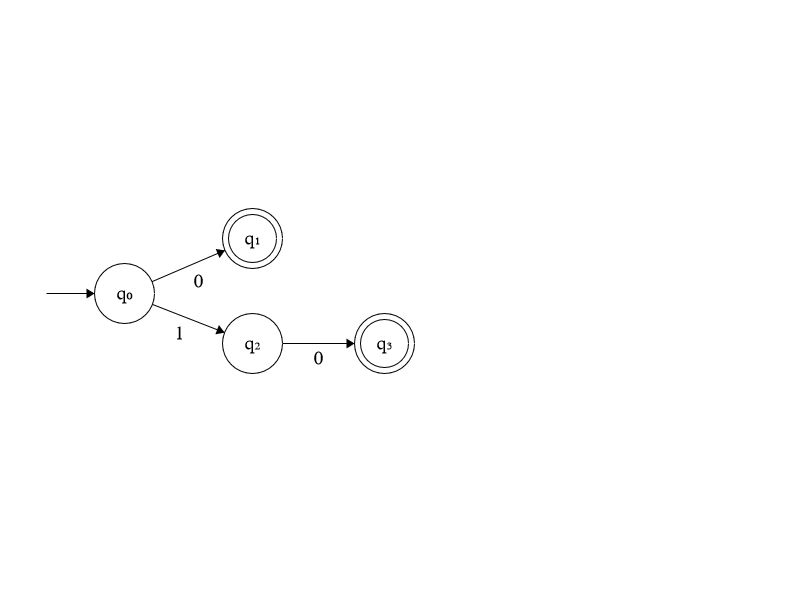
\includegraphics[width=\textwidth]{Immagini/L2.jpeg}
\caption{L2}
\label{fig:L2}
\end{subfigure}
\label{fig:combined}
\end{figure}

